\documentclass{article}
\usepackage{amsmath}
\usepackage{graphicx}

\begin{document}

\section*{Figuring out what happens with the solver
  \centering when there is attenuation}

I like to use simple test cases because they clarify to me what is
\textit{not} the problem. So I will be considering the following
situation: a $1\times 1\times 1$ meter box, and I will be evaluating
the solution at the center of that cube. The left face of the cube is
marked as a port, as is the right. So the equations we will be
solving when we are driving the left port are:
\begin{align*}
  -\omega^2 p(x,y,z) - c^2 \Delta p(x,y,z) &= 0, \\
  p(x=0,y,z) &= 1, && \text{(left boundary)}\\
  p(x=1,y,z) &= 0, && \text{(right boundary)} \\
    \frac{\partial p}{\partial n} &= 0,
     && \text{(all other boundaries)}
\end{align*}
The wave speed is computed as
\begin{align*}
  c = \sqrt{\frac{K}{\rho}},
\end{align*}
where $K$ is the bulk modulus and $\rho$ is the density, both of which
are read from the input file as frequency-dependent quantities, and
which can both be complex-valued.


\section{Testing the pressure}

The set-up is chosen so that the solution is one-dimensional. As a
consequence, the solution only depends on $x$ and we can easily derive
it as
\begin{align*}
  p(x,y,z) = p(x) &= \frac{e^{jkx} - e^{-jk(2L-x)}}{1 - e^{-2jkL}},
\end{align*}
with $L=1$ and $k=\frac{\omega}{c}$. It is not difficult to verify
that indeed the boundary conditions are satisfied:
\begin{align*}
  p(0) &= \frac{e^{jk0} - e^{-jk(2L-0)}}{1 - e^{-2jkL}}
  =
  \frac{1 - e^{-2jkL}}{1 - e^{-2jkL}} = 1,
  \\
  p(L) &= \frac{e^{jkL} - e^{-jk(2L-L)}}{1 - e^{-2jkL}}
  = \frac{e^{jkL} - e^{-jkL}}{1 - e^{-2jkL}} = 0.
\end{align*}
It is also not difficult to check that the equation itself is
satisfied:
\begin{align*}
  -\omega^2 p(x) - c^2 \Delta p(x)
  &= -\omega^2 p(x) - c^2 p''(x)\\
  &= -\omega^2 p(x) - c^2 (jk)^2 p''(x)  \\
  &= (k^2c^2-\omega^2) p(x) \\
  &= \left(\frac{\omega^2}{c^2}c^2-\omega^2\right) p(x)\\
  &= 0.
\end{align*}

With this solution, evaluated at the center of the box of length
$L=1$, we obtain
\begin{align*}
  p_\text{center} &= p(0.5)
  \\
  &= \frac{e^{\frac{jk}{2}} - e^{-\frac{3jk}{2}}}{1 - e^{-2jk}}
  \\
  &= \frac{e^{\frac{jk}{2}} - e^{-\frac{3jk}{2}}}{e^{jk} - e^{-jk}}
  \\
  &= \frac{e^{\frac{j\omega}{2c}} - e^{-\frac{3j\omega}{2c}}}{1 - e^{-\frac{2j\omega}{c}}}
  \\
  &= \frac{e^{\frac{j\omega}{2}\sqrt{\frac{\rho}{K}}} - e^{-\frac{3j\omega}{2}\sqrt{\frac{\rho}{K}}}}{1 - e^{-2j\omega\sqrt{\frac{\rho}{K}}}}
\end{align*}
We will consider this expression for two special cases below, without
and with attenuation.


\subsection{No attenuation}

Let us consider the evaluation of the pressure at the center of the
box for the special case without attenuation. For simplicity, we
choose $\rho=K=1$ and consequently $c=1$ and $k=\omega$. Then, based
on the formulas in the \texttt{readme.md} file at the top level of the
github repository, we have
\begin{align*}
  p(x)
  &=
  \frac{e^{jkx} - e^{-jk(2L-x)}}{1 - e^{-2jkL}}.
\end{align*}
This formula, after a good bit of massaging, can be restated as
follows for real-valued $k$:
\begin{align*}
  p(x)
  &=
  \frac{\sin(k(L-x))}{\sin(kL)}.
  \\
  &=
  \frac{\sin(\omega(1-x))}{\sin(\omega)}.
\end{align*}
This expression, unsurprisingly, has singularities for
$\omega=\pi,2\pi,3\pi,...$, where the cavity is in resonance. This
corresponds to frequencies $f=0.5, 1, 1.5, \ldots$ Hertz. As a
consequence, we better consider frequences below the first resonance,
i.e., $\omega<\pi$, i.e., $f<0.5$ Hertz.

That said, for the specific case of the center of the box (at $x=0.5$), we get
\begin{align*}
  p_\text{center}
  &= 
  \frac{\sin(\omega/2)}{\sin(\omega)}.
\end{align*}
In the low-frequency case, $\omega\ll 1$, we have the asymptotic
behavior $\sin(t)\approx t$ and so
\begin{align*}
  p_\text{center}
  &\approx
  \frac{\omega/2}{\omega}
  = \frac 12.
\end{align*}
This makes sense: In the low-frequency limit, the length of the cavity
is much less than the wavelength and so the pressure simply decreases
linearly from one at the left end to zero at the right end -- implying
a pressure of 0.5 at the center of the object.

We can plot what the program produces for a number of frequencies in
the range between 0.01 and 1 Hz:
%
% dii_frequency_response.csv, columns 1 (frequency), 14 (real part of
% pressure), 15 (imaginary part of pressure)
%

\begin{center}
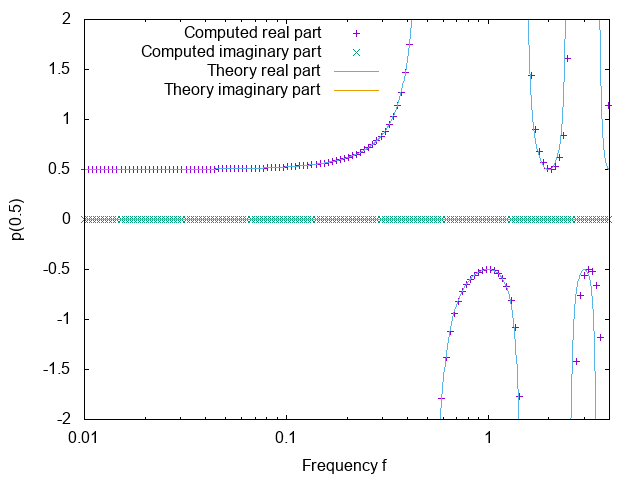
\includegraphics[width=0.7\textwidth]{unit-cube/no-attenuation/pressure-at-center.png}
\end{center}

As can be seen, the computations (shown as the purple and green crosses)
are an excellent match for the expected theoretical behavior, at least
in the low-frequency regime. Furthermore, the singularity (resonance)
is at $f=0.5$ Hz, again as expected. (For higher frequencies, the
crosses are no longer a good fit, but this is because we compute on a
mesh that has only $4\times 4\times 4$ cells. We can not expect it to
accurately resolve the solution for frequencies $f\ge 4$ where the
wavelength $\lambda=c/f$ drops below the cell diameter.)


\subsection{With attenuation}

Let us now consider the case with attenuation. Specifically, we will
choose the same box of length $L=1$, but use $\rho=1-j, K=1$ and
consequently $c=\sqrt{\frac{K}{\rho}}=\sqrt{\frac{1}{1-j}}=\frac{1}{2^{1/4}}e^{j\pi/8}$ 
and $k=\omega/c=2^{1/4}e^{-j\pi/8} \omega$. Then, again based
on the formulas in the \texttt{readme.md} file at the top level of the
github repository, we have
\begin{align*}
  p(x)
  &=
  \frac{e^{jk(L-x)} - e^{-jk(L-x)}}{e^{jkL} - e^{-jkL}}.
\end{align*}
This time, because $k$ is not real valued, we cannot replace $e^{ja}$
by $\cos(a)+j\sin(a)$, and instead need to use the expression as
is. We can, however, simplify it to
\begin{align*}
  p(x)
  &=
  \frac{\sinh(jk(L-x))}{\sinh(jkL)}.
\end{align*}
Consequently,
\begin{align*}
  p_\text{center}
  &=
  \frac{\sinh(jk/2))}{\sinh(jk)}.
\end{align*}
We can again make the same observation that in the low-frequency
limit, $\sinh(t)=\frac 12(e^t-e^{-t})\approx \frac 12[(1+t)-(1-t)]=t$,
and so
\begin{align*}
  p_\text{center}
  &=
  \frac{\sinh(jk/2))}{\sinh(jk)}
  \approx
  \frac{jk/2}{jk}
  = \frac 12.
\end{align*}
The reasoning for this is as before: With or without damping, in the
low-frequency regime, the pressure is linear and so equal to one half
at the center of the domain.

We can again output the results of our computations:
\begin{center}
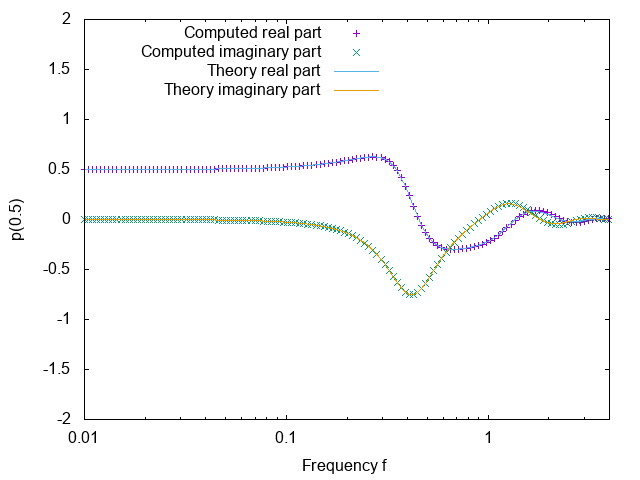
\includegraphics[width=0.7\textwidth]{unit-cube/with-attenuation/pressure-at-center.png}
\end{center}
As before, the results provide an excellent match to the theoretical expectations.


\section{Testing the velocity}

We can also look at the velocity at the center point. The velocity is
defined as $\mathbf u(\mathbf x)=j\omega \nabla p(\mathbf x)$ but
because everything only depends on the $x$ coordinate, only one
component of the velocity is nonzero and we can simply denote it by
(non-bold) $u(x)=-\frac{1}{j\rho\omega}\frac{d}{dx} p(x)$.

\subsection{No attenuation}

With the expression for the pressure above for the case without
attenuation, we get
\begin{align*}
  u(x)
  &=
  -\frac{1}{j\rho\omega} \frac{d}{dx} \frac{\sin(\omega(1-x))}{\sin(\omega)}
  \\
  &=
  -\frac{1}{j\rho} \frac{-\cos(\omega(1-x))}{\sin(\omega)},
\end{align*}
and consequently
\begin{align*}
  u_\text{center}
  &=
  \frac{1}{j\rho} \frac{\cos(\omega/2)}{\sin(\omega)}
  \\
  &=
  -\frac{j}{\rho} \frac{\cos(\omega/2)}{\sin(\omega)}.
\end{align*}
In the low-frequency regime, this expression has the asymptotic behavior
\begin{align*}
  u_\text{center}
  &\approx
  -\frac{j}{\rho} \frac{1}{\omega}.
\end{align*}


We can again compare this against what the program computes:
\begin{center}
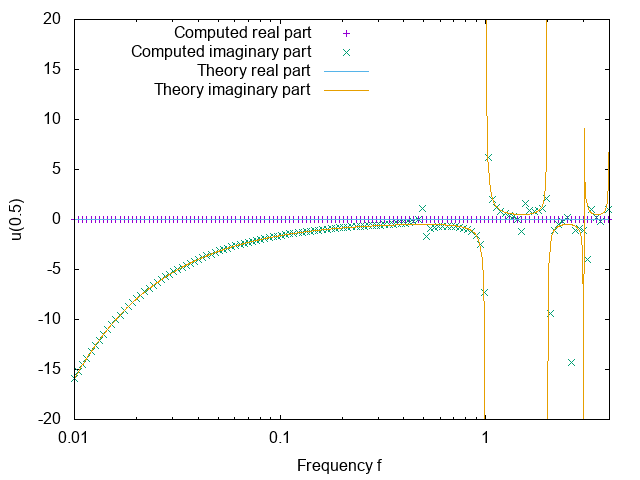
\includegraphics[width=0.7\textwidth]{unit-cube/no-attenuation/velocity-at-center.png}
\end{center}
As before, in the low-frequency range, the agreement is
excellent. (And, as before, the agreement is not good in the
high-frequency range because the mesh is too coarse. There is also a
little blip at the first resonance at $f=0.5$ Hz. This is because
while the pressure becomes very large at the resonance, the
\textit{exact} velocity stays bounded -- but the numerical
approximation becomes poor.)

While not shown
in the figure, one can easily check that the asymptotic behavior
outlined above is also respected by the actual computed data points.



\subsection{With attenuation}

For the case with attenuation, let us start with
\begin{align*}
  p(x)
  &=
  \frac{\sinh(jk(L-x))}{\sinh(jkL)},
\end{align*}
to compute
\begin{align*}
  u(x)
  &=
  -\frac{1}{j\rho\omega} \frac{d}{dx}
  \frac{\sinh(jk(L-x))}{\sinh(jkL)}
  \\
  &=
  -\frac{1}{j\rho\omega}
  \frac{-jk\cosh(jk(L-x))}{\sinh(jkL)}
  \\
  &=
  \frac{k}{\rho\omega}
  \frac{\cosh(jk(L-x))}{\sinh(jkL)}
  \\
  &=
  \frac{1}{\rho c}
  \frac{\cosh(jk(L-x))}{\sinh(jkL)}
  \\
  &=
  \frac{1}{\rho}\sqrt{\frac{\rho}{K}}
  \frac{\cosh(jk(L-x))}{\sinh(jkL)}
  \\
  &=
  \frac{1}{\sqrt{\rho K}}
  \frac{\cosh(jk(L-x))}{\sinh(jkL)}.
\end{align*}
From this we then get
\begin{align*}
  u_\text{center}
  &=
  \frac{1}{\sqrt{\rho K}}
  \frac{\cosh(jk/2)}{\sinh(jk)}.
\end{align*}
In the low-frequency regime, the asymptotic expansion of this
expression is
\begin{align*}
  u_\text{center}
  &\approx
  \frac{1}{\sqrt{\rho K}}
  \frac{1}{jk}
  =
  -\frac{j}{\sqrt{\rho K}}
  \frac{\sqrt{K}}{\omega\sqrt{\rho}}
  =
  -\frac{j}{\omega\rho}.
\end{align*}
This is the same expression as for the case without attenuation,
except that now $\rho$ may be complex-valued.

If we compare the exact expression against computations, we obtain the
following figure:
\begin{center}
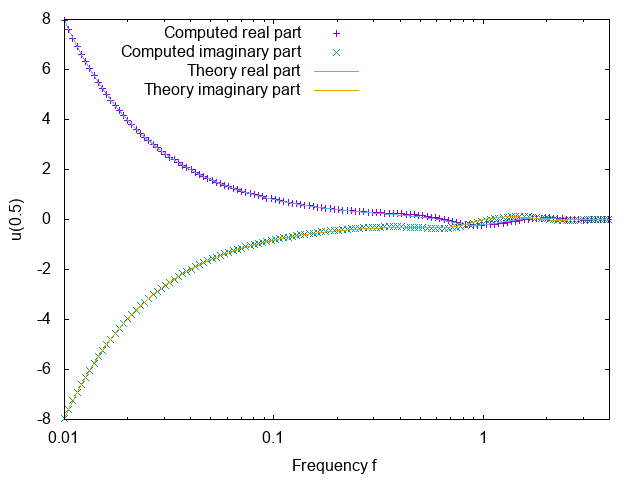
\includegraphics[width=0.7\textwidth]{unit-cube/with-attenuation/velocity-at-center.png}
\end{center}
The match is again excellent.


\section{On a small, rectangular wave guide}

The original report of results that deviate from those that are
expected were for a small rectangular wave guide of size 5mm by 5mm by
10mm. We can adapt the case above to the same situation
here. Specifically,the solution in general is given by
\begin{align*}
  p(x)
  &=
  \frac{\sinh(jk(L-x))}{\sinh(jkL)},
  \\
  u(x)
  &=
  \frac{1}{\sqrt{\rho K}}
  \frac{\cosh(jk(L-x))}{\sinh(jkL)}.
\end{align*}
We set $L=0.01$ (10mm), and recall $k=\frac{\omega}{c}=\sqrt{\frac{K}{\rho}}\omega$.

\end{document}
